\documentclass{sigchi}

% Copyright
\CopyrightYear{2019}
\setcopyright{acmlicensed}

% Load basic packages
\usepackage{balance}       % to better equalize the last page
\usepackage{graphics}      % for EPS, load graphicx instead 
\usepackage[T1]{fontenc}   % for umlauts and other diaeresis
\usepackage{txfonts}
\usepackage{mathptmx}
\usepackage[pdflang={en-US},pdftex]{hyperref}
\usepackage{color}
\usepackage{booktabs}
\usepackage{textcomp}

% Some optional stuff you might like/need.
\usepackage{microtype}        % Improved Tracking and Kerning
% \usepackage[all]{hypcap}    % Fixes bug in hyperref caption linking
\usepackage{ccicons}          % Cite your images correctly!
% \usepackage[utf8]{inputenc} % for a UTF8 editor only

\usepackage{todonotes}

% Paper metadata (use plain text, for PDF inclusion and later
% re-using, if desired).  Use \emtpyauthor when submitting for review
% so you remain anonymous.
\def\plaintitle{Detecção de Malária usando Redes Neurais Convolucionais}

% llt: Define a global style for URLs, rather that the default one
\makeatletter
\def\url@leostyle{%
  \@ifundefined{selectfont}{
    \def\UrlFont{\sf}
  }{
    \def\UrlFont{\small\bf\ttfamily}
  }}
\makeatother
\urlstyle{leo}

% To make various LaTeX processors do the right thing with page size.
\def\pprw{8.5in}
\def\pprh{11in}
\special{papersize=\pprw,\pprh}
\setlength{\paperwidth}{\pprw}
\setlength{\paperheight}{\pprh}
\setlength{\pdfpagewidth}{\pprw}
\setlength{\pdfpageheight}{\pprh}

% Make sure hyperref comes last of your loaded packages, to give it a
% fighting chance of not being over-written, since its job is to
% redefine many LaTeX commands.
\definecolor{linkColor}{RGB}{6,125,233}
\hypersetup{%
  pdftitle={\plaintitle},
% Use \plainauthor for final version.
%  pdfauthor={\plainauthor},
  pdfauthor={\emptyauthor},
  pdfkeywords={\plainkeywords},
  pdfdisplaydoctitle=true, % For Accessibility
  bookmarksnumbered,
  pdfstartview={FitH},
  colorlinks,
  citecolor=black,
  filecolor=black,
  linkcolor=black,
  urlcolor=linkColor,
  breaklinks=true,
  hypertexnames=false
}

% End of preamble. Here it comes the document.
\begin{document}

\title{\plaintitle}

\numberofauthors{5}
\author{%
{Anderson Silva, Bruno Pospichil, Diego Rosso, Júlio Pires, Pedro Dutra }
}

\maketitle

\begin{abstract}\
\begin{quote}
Este artigo descreve o trabalho final da disciplina de Deep Learning I, sendo escolhido pelo grupo um problema de classificação em visão computacional com foco na detecção de malária em um dataset composto por imagens de gotas de sangue de pacientes - infectados ou não - em uma lâmina microscópica feita em laboratório. Por ser um problema de classificação de imagens, foi selecionado o uso de redes neurais convolucionais para resolução desta tarefa.
\end{quote}
\end{abstract}

\section{Introdução}
Conforme a Organização Mundial da Saúde (OMS) \cite{WHO}, uma agência subordinada à ONU, a malária é uma doença febril aguda com um período de incubação de 7 dias ou mais. É uma doença evitável e curável, porém, com risco de óbito, sendo transmitida pelos mosquitos fêmeas Anopheles - comumente chamado mosquito-prego no Brasil - infectados pelo parasita Plasmodium. Entre as características clínicas variáveis incluem febre, calafrios, dor de cabeça, dor e fraqueza muscular, vômitos, tosse, diarreia e dor abdominal. Outros sintomas incluem à falência de órgãos, como insuficiência renal, edema pulmonar, convulsões generalizadas, colapso circulatório, seguidos de coma e morte.

Dado a importância e relevância deste problema, optamos por buscar solucionar este desafio usando aprendizagem profunda com redes neurais convolucionais. Neste sentido, foi selecionado o framework \textbf{PyTorch} e, dado o problema de detecção de malária através de imagens ser um desafio de visão computacional, foi escolhido o uso de Redes Neurais Convolucionais (CNN). O dataset é composto por 27558 imagens, sendo balanceado entre amostras infectadas e saudáveis. As imagens estão no formato PNG e em formato RGB com 3 canais de cores.

Como proposta de solução deste problema de classificação binária (célula infectada x saudável), foram desenvolvidas três abordagens distintas visando explorar as características das redes neurais convolucionais, suas respectivas arquiteturas e hiperparâmetros: Abordagem I) AlexNet: Treinamento do dataset do zero da arquitetura sem o uso de técnicas de transfer learning (fine-tuning ou extração de features); Abordagem II) AlexNet: treinamento da arquitetura com o uso da técnica de fine-tuning, Abordagem III) ResNet50: Uso de uma arquitetura mais profunda e atual, utilizando técnica de fine-tuning para o mesmo problema.

\section{Tratamento Inicial das Imagens}
As imagens contidas no conjunto de dados possuem tamanhos variados, onde cada imagem possui uma variação distinta entre a respectiva largura e altura comparada com as demais, o que tende a ser um problema para a etapa de treinamento. Desta forma, optamos por normalizar o tamanho utilizando a transformação \textit{Resize} do PyTorch, onde as imagens são redimensionadas para o mesmo tamanho, definido como 256x256. Foi criado também uma classe, nomeada como MalariaDataset, visando carregar as imagens do dataset, respeitando a respectiva organização das pastas ['Parasitized', 'Uninfected'].

\section{Protocolo de treino, validação e teste}
Como parte do protocolo de avaliação da rede, o dataset de imagens foi separado em 3 conjuntos distintos: treino, teste e validação. No conjunto de imagens de treino foi utilizado 60\% das imagens (19292 amostras), 15\% para teste (4133 amostras) e 15\% para validação (4133 amostras). Os ajustes nos hiperparâmetros foram efeitos apenas nas etapas de treino e validação. Foram utilizados também um batch size de 32 e um processo de treinamento com 10 épocas. E como otimizador foi utilizado SGD. Para o cálculo de \texti{loss} foi utilizado a função de entropia cruzada.

\section{Arquiteturas abordadas}
Neste trabalho foram desenvolvidas três abordagens utilizando redes convolucionais para o problema de detecção de malária. No primeiro momento, foi utilizada a arquitetura da AlexNet com o processo de treinamento feito do zero. A ideia era avaliar a capacidade da arquitetura pra a resolução do problema proposto e compará-la com outras abordagens.

\subsection{I. Arquitetura AlexNet: Treinamento completo}
Como intuição inicial, optamos por realizar a detecção de malária com a arquitetura AlexNet, rede neural convolucional vencedora do desafio \textit{ImageNet Visual Recognition} em 2012. Nesta abordagem, foi utilizada a arquitetura da AlexNet para treinar todo o modelo - sem o uso de técnicas de transfer learning e fine-tuning. O objetivo era entender as diferenças e os impactos de um treinamento completo em comparação com técnicas de transfer learning/fine tuning e a respectiva inicialização dos pesos.

Neste sentido, através do PyTorch utilizamos a AlexNet com o parâmetro pretrained como false. Por ser um problema binário, ajustamos a camada linear visando a classificação de duas classes, visto a rede ter sido desenvolvida originalmente para as 1000 classes do ImageNet.

\begin{figure}[ht!]
\centering
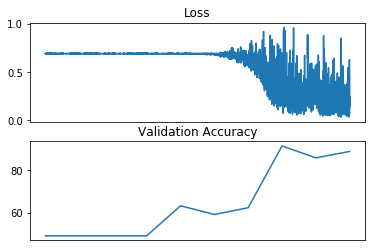
\includegraphics[scale=0.5]{./figures/alexnet.png}
\caption{Validação - AlexNet: Treinamento completo}
\label{fig:alexnet}
\end{figure}

\subsection{II. Arquitetura AlexNet: Fine-Tuning}
Nesta seção, em contraste com a anterior, é descrita a utilização da técnica de fine-tuning de uma instância da arquitetura da AlexNet já pré-treinada, aproveitando os respectivos pesos da rede como parte do processo de treinamento. Assim como a abordagem anterior, foi ajustado a última camada do classificador linear para um problema de 2 classes.

\begin{figure}[ht!]
\centering
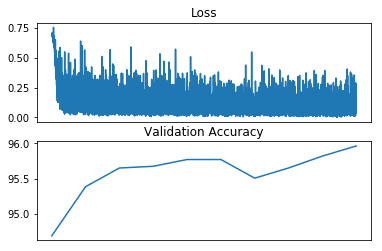
\includegraphics[scale=0.5]{./figures/alexnet-finetunning.png}
\caption{Validação - AlexNet: Fine-tuning}
\label{fig:alexnet-finetuning}
\end{figure}

\subsection{III. Arquitetura ResNet50}
Como um contraponto em relação aos dois experimentos realizados com a AlexNet, foi também utilizada a ResNet50, uma rede mais profunda e atual. Neste cenário, foi utilizado o modelo do PyTorch com o pretrained ativado. Como parte do processo de fine-tuning, foi ajustado a camada fully connected para um problema de 2 classes - originalmente 1000.

No processo de treinamento da ResNet50, observamos um tempo superior a AlexNet no treino de cada batch de imagens entre as épocas. Como intuição, acreditamos que seja devido a arquitetura da ResNet50 ser mais profunda que a AlexNet - enquanto a AlexNet possui 5 camadas convolucionais e 3 camadas fully-connected, a ResNet possui 50 camadas.


\begin{figure}[ht!]
\centering
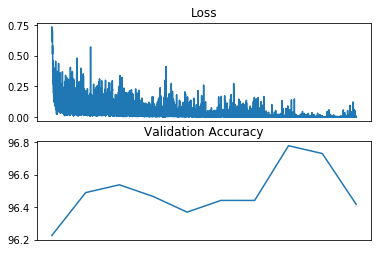
\includegraphics[scale=0.5]{./figures/resnet50.png}
\caption{Validação - ResNet: Fine-tuning}
\label{fig:resnet-finetuning}
\end{figure}

\section{Discussões}

Seguindo o processo de treinamento, validação e teste, observamos os seguintes aspectos nos 3 experimentos usando Redes Neurais Convolucionais: 
\item{I) \textbf{Treinamento completo:} Ao utilizar uma arquitetura com treinamento completo, isto é, não sendo pré-treinada, a rede acaba demorando um conjunto de épocas até convergir em uma boa precisão sobre o conjunto de validação. Dependendo do problema, talvez não seja uma opção interessante. }

\item{II) \textbf{Fine-tuning:} O uso de uma rede pré-treinada, tornou-se possível observar que em poucas épocas a rede já conseguia atingir bons resultados, uma técnica que torna interessante para aumentar a velocidade e otimizar o processo de treinamento.} 

\item{III) \textbf{Otimizadores:} Abordamos neste trabalho o Adam e o Gradiente Descendente Estocástico com momentum. Previamente, nossa expectativa era que o Adam tivesse um resultado melhor no processo de otimização e convergência em relação ao SGD. Porém, ao realizarmos simulações com ambos, observamos que o SGD com momentum teve um resultado superior ao Adam. Foi utilizado um momentum de 0.9.
}

\item{III) \textbf{Learning Rate:} Observamos resultados interessantes com uma taxa de aprendizagem de 0.001 nas redes com fine-tuning - AlexNet e ResNet50. Porém, na AlexNet, em um treinamento completo, ocorre pouca variação no loss e accuracy nas primeiras épocas, estabilizando apenas após estes saltos iniciais.
}
\section{Resultados}

A tabela-1 mostra o valor de acurácia das redes na décima época de treino e o resultado da acurácia do modelo contra dataset de teste o qual não foi utilizado durante o treino e validação.

\begin{table}[ht!]
\begin{tabular}{|l|l|l|}
\hline
\thead{Rede convolucional} & \thead{Acurácia validação} & \thead{Acurácia teste}  \\ \hline
\multicolumn{1}{|l|}{AlexNet}               & 88.89  & 89.56  \\ \hline
\multicolumn{1}{|l|}{AlexNet Fine Tunning}  & 95.96  & 95.60  \\ \hline
\multicolumn{1}{|l|}{ResNet50}              & 96.42  & 96.25  \\ \hline
\end{tabular}
\caption{Comparativo de resultados}
\end{table}

\section{Conclusão}
O estado da arte para este problema no artigo \cite{rajaraman2019performance} possui alguns resultados interessantes: 1) Uso de Ensemble Learning 99.5\% \cite{rajaraman2019performance}, 2) GoogLenet/Inception 98.1\% \cite{dong2017evaluations} e 3) 97.7\% \cite{gopakumar2018convolutional}. Em nosso trabalho, utilizando o protocolo de treino, validação e teste, foi possível atingir 96.25\% sendo um resultado próximo ao estado da arte para o problema. 

% BALANCE COLUMNS
\balance{}

% REFERENCES FORMAT
% References must be the same font size as other body text.
\bibliographystyle{SIGCHI-Reference-Format}
\bibliography{sample}

\end{document}